% Pappus chain in the arbelos, AB=1, AC=0.62: the n-th circle has radius t(1-t)/(2(t+n^2(1-t)^2)) and centre at height 2n r_n.
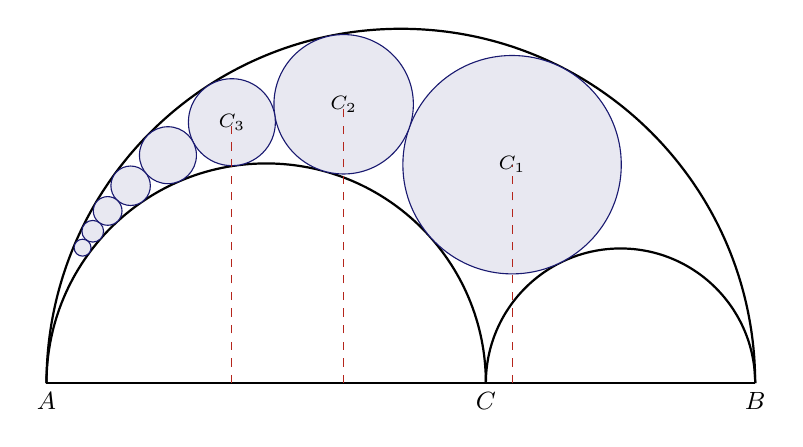
\begin{tikzpicture}[font=\small]
\draw[thick] (0.000,0) arc (180:0:4.500);
\draw[thick] (0.000,0) arc (180:0:2.790);
\draw[thick] (5.580,0) arc (180:0:1.710);
\draw[thick] (0,0) -- (9.000,0);
\draw[MidnightBlue,fill=MidnightBlue!10] (5.9129,2.7739) circle (1.3870);
\draw[BrickRed,dashed] (5.9129,0) -- (5.9129,2.7739);
\node[font=\scriptsize] at (5.9129,2.7739) {$C_1$};
\draw[MidnightBlue,fill=MidnightBlue!10] (3.7740,3.5411) circle (0.8853);
\draw[BrickRed,dashed] (3.7740,0) -- (3.7740,3.5411);
\node[font=\scriptsize] at (3.7740,3.5411) {$C_2$};
\draw[MidnightBlue,fill=MidnightBlue!10] (2.3546,3.3138) circle (0.5523);
\draw[BrickRed,dashed] (2.3546,0) -- (2.3546,3.3138);
\node[font=\scriptsize] at (2.3546,3.3138) {$C_3$};
\draw[MidnightBlue,fill=MidnightBlue!10] (1.5424,2.8943) circle (0.3618);
\draw[MidnightBlue,fill=MidnightBlue!10] (1.0685,2.5064) circle (0.2506);
\draw[MidnightBlue,fill=MidnightBlue!10] (0.7768,2.1866) circle (0.1822);
\draw[MidnightBlue,fill=MidnightBlue!10] (0.5873,1.9287) circle (0.1378);
\draw[MidnightBlue,fill=MidnightBlue!10] (0.4583,1.7201) circle (0.1075);
\node[below] at (0,0) {$A$};
\node[below] at (5.580,0) {$C$};
\node[below] at (9.000,0) {$B$};
\end{tikzpicture}
